\section{Vulnerability Analysis and Reference-System Validation}
\label{sec:reference-validation}

\graphicspath{{../evidence/}{evidence/}}

Chapter~3 established VM~270 \code{copyfail01} as the clean reference system.
That baseline answers what was installed and running, but it does not answer the
next question: could this exact state reproduce Copy Fail? A 6.8-series kernel,
the AF\_ALG subsystem, or an \code{algif\_aead} file on disk is not enough on
its own. The interface must be supported, reachable at runtime, and backed by a
kernel that still contains the vulnerable behaviour.

This chapter checks those conditions without running the proof of concept on
VM~270. That boundary is deliberate. If the reference system is already
protected, downgrading it or removing its mitigation would destroy the most
useful comparison state in the laboratory. The result of this analysis therefore
decides whether VM~270 can be used directly or whether the vulnerable state has
to be reconstructed on the separate experimental clone, VM~271.

\begin{evidencebox}
Phase~01 is stored under
\path{evidence/01-vulnerability-validation/}. The public set contains seven
text artifacts and seven screenshots. An independent check of
\path{PUBLIC-SHA256SUMS} verified all 14 listed objects with no failures. The
machine-readable captures remain the primary evidence; selected screenshots are
included here to make the decisive states visible in the report.
\end{evidencebox}

\subsection{Validation Question and Method}

The validation was organised around five separate questions:

\begin{enumerate}
    \item Does the installed kernel provide the \code{algif\_aead} module?
    \item Is the AF\_ALG AEAD userspace interface enabled in the running
          kernel's configuration?
    \item Was \code{algif\_aead} loaded when the evidence was collected?
    \item What does the ordinary \code{modprobe} path do when the module is
          requested?
    \item Is the active Ubuntu kernel before or after Canonical's published
          fixed-package boundary?
\end{enumerate}

Keeping these questions separate prevents several misleading shortcuts. A
module can exist without being loaded. Kernel support can be configured while a
distribution policy blocks normal loading. Even a reachable interface does not
establish vulnerability if the active implementation is already corrected.
Suitability for reproduction depends on the combined state, not on a single
command or version string.

The seven textual artifacts record the running kernel, relevant package
versions, module metadata, kernel configuration, effective loading policy, and
runtime module state. They are interpreted below in that order. No exploit was
executed on VM~270 during this phase, so the result is a prerequisite assessment
rather than an exploit-success or exploit-failure experiment.

\clearpage

\subsection{Module Object and Kernel Configuration}

The capture in \path{03-algif-aead-modinfo.txt} shows that the running kernel's
module tree contains \code{algif\_aead}:

\begin{lstlisting}
filename: /lib/modules/6.8.0-137-generic/kernel/crypto/algif_aead.ko.zst
description: AEAD kernel crypto API user space interface
depends: af_alg
intree: Y
name: algif_aead
vermagic: 6.8.0-137-generic SMP preempt mod_unload modversions
\end{lstlisting}

The filename and \code{vermagic} associate the object with the active
\code{6.8.0-137-generic} release. Its description identifies the AEAD
userspace interface relevant to Copy Fail, while the dependency on
\code{af\_alg} matches the AF\_ALG path described in Chapter~1.

The corresponding configuration capture in \path{04-kernel-config.txt}
contains:

\begin{lstlisting}
CONFIG_CRYPTO_USER_API=m
CONFIG_CRYPTO_USER_API_HASH=m
CONFIG_CRYPTO_USER_API_SKCIPHER=m
CONFIG_CRYPTO_USER_API_RNG=m
# CONFIG_CRYPTO_USER_API_RNG_CAVP is not set
CONFIG_CRYPTO_USER_API_AEAD=m
# CONFIG_CRYPTO_USER_API_ENABLE_OBSOLETE is not set
\end{lstlisting}

The decisive entry is \code{CONFIG\_CRYPTO\_USER\_API\_AEAD=m}. The value
\code{m} means that this userspace AEAD interface is available as a loadable
module rather than omitted or built directly into the kernel. This agrees with
the module object reported by \code{modinfo}.

\begin{figure}[H]
    \centering
    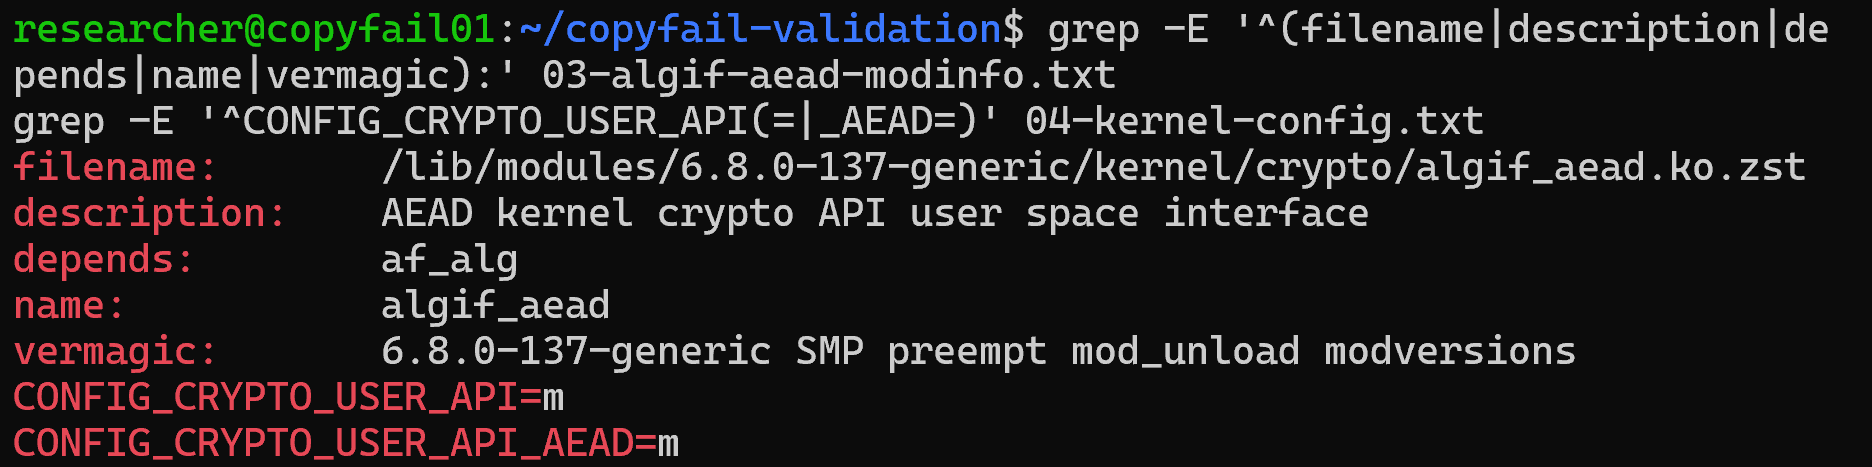
\includegraphics[
        width=\textwidth,
        height=0.31\textheight,
        keepaspectratio
    ]{01-vulnerability-validation/screenshots/04-algif-aead-module-and-kernel-config.png}
    \caption{Phase~01 capture linking the installed \code{algif\_aead} object
    to the active kernel and showing modular AEAD userspace support.}
    \label{fig:phase01-module-config}
\end{figure}

These observations establish installed capability only. Neither \code{modinfo}
nor the kernel configuration proves that the module was loaded, that the normal
loading path would permit it, or that its implementation remained vulnerable.
Those properties require the runtime, policy, and package checks that follow.

\subsection{Runtime Module State}

The loaded-module list was checked with an exact-name query:

\begin{lstlisting}
lsmod | grep '^algif_aead\b'
\end{lstlisting}

The command returned no output. For that reason,
\path{07-module-loaded.txt} is exactly zero bytes; it is not a missing capture.
Its manifest entry uses the standard SHA-256 digest of an empty file:

\begin{lstlisting}
e3b0c44298fc1c149afbf4c8996fb92427ae41e4649b934ca495991b7852b855  07-module-loaded.txt
\end{lstlisting}

The accompanying screenshot uses a human-readable conditional wrapper and
prints \code{algif\_aead is NOT currently loaded}. It presents the same point-in-
time result without replacing the machine-readable empty artifact.

\begin{figure}[H]
    \centering
    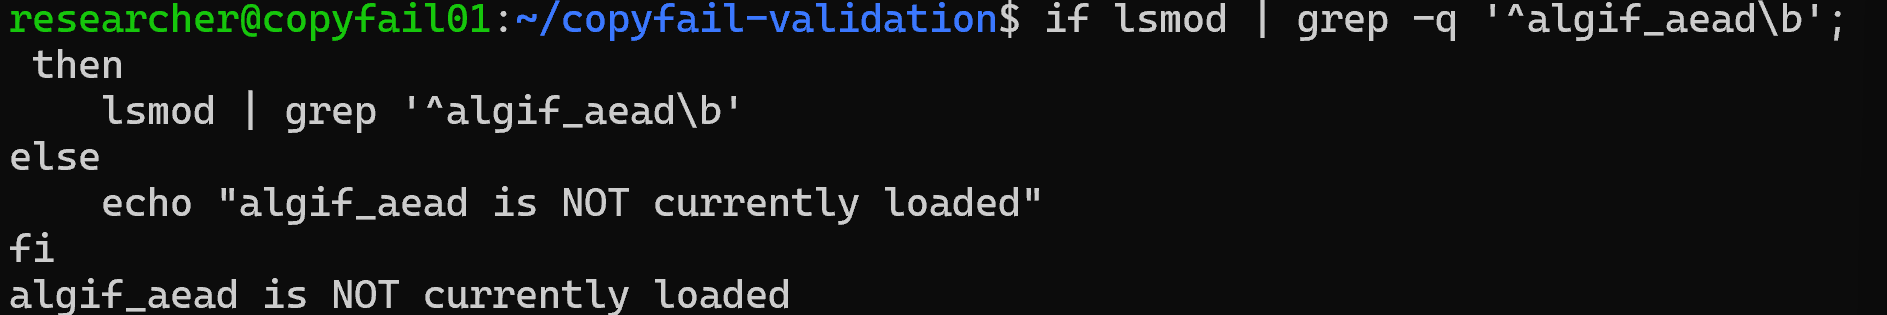
\includegraphics[
        width=\textwidth,
        height=0.29\textheight,
        keepaspectratio
    ]{01-vulnerability-validation/screenshots/05-algif-aead-not-loaded.png}
    \caption{Runtime check showing that \code{algif\_aead} was not loaded at
    the Phase~01 collection point.}
    \label{fig:phase01-module-unloaded}
\end{figure}

This result is intentionally narrow. It proves that the module did not appear
in the loaded-module list at that moment. By itself, it cannot distinguish a
module that had simply not been requested from one whose loading was actively
blocked. The effective policy check supplies that missing context.

\subsection{Effective Module-Loading Policy}

The capture in \path{05-modprobe-config.txt} found the following rule:

\begin{lstlisting}
/etc/modprobe.d/disable-algif_aead.conf:1:# Disable algif_aead module due to CVE-2026-31431 (AKA copy.fail)
/etc/modprobe.d/disable-algif_aead.conf:5:install algif_aead /bin/false
\end{lstlisting}

For \code{modprobe}, the \code{install} directive replaces normal insertion of
the named module with the specified command. Here, a request for
\code{algif\_aead} is redirected to \code{/bin/false}, which exits
unsuccessfully without inserting the module. Canonical documents the same
\code{kmod}-based rule as a temporary Copy Fail mitigation
\cite{ubuntu-copyfail-cve,ubuntu-copyfail-fixes}.

The configuration was not interpreted from the file alone. The effective path
was resolved with a dry run and preserved in
\path{06-modprobe-dry-run.txt}:

\begin{lstlisting}
insmod /lib/modules/6.8.0-137-generic/kernel/crypto/af_alg.ko.zst
install /bin/false
\end{lstlisting}

The first line resolves the \code{af\_alg} dependency. The second shows that
the requested \code{algif\_aead} insertion resolves to the replacement command
instead of an \code{insmod} operation.

\begin{figure}[H]
    \centering
    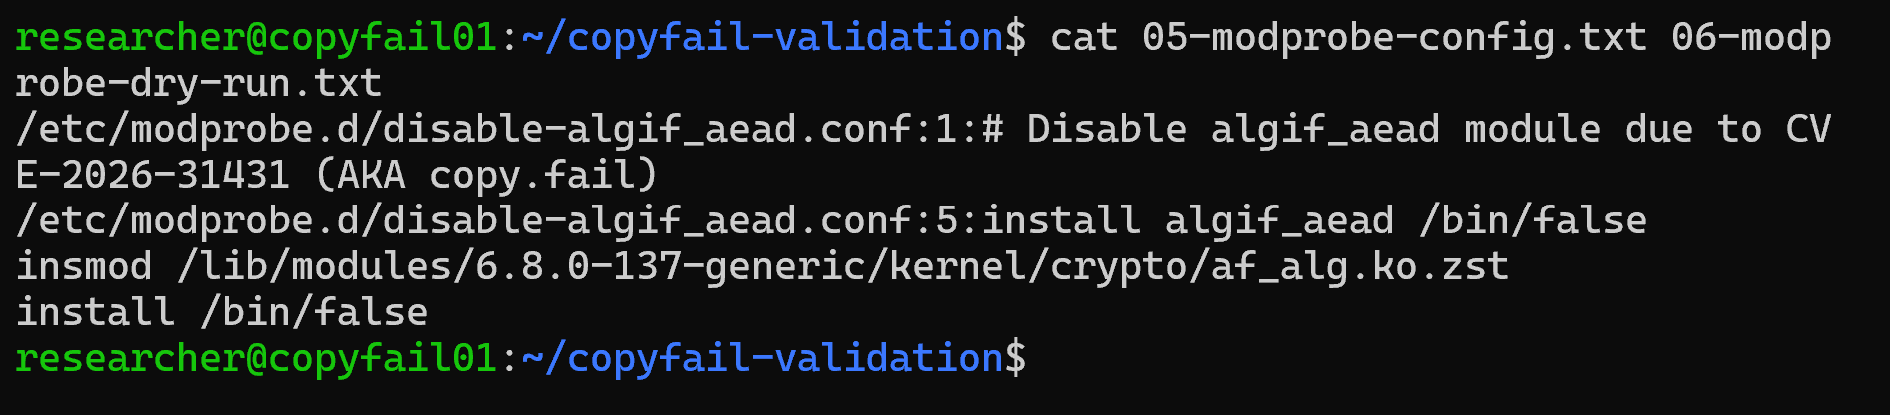
\includegraphics[
        width=\textwidth,
        height=0.31\textheight,
        keepaspectratio
    ]{01-vulnerability-validation/screenshots/03-algif-aead-mitigation-active.png}
    \caption{Configuration and dry-run output showing the active
    \code{algif\_aead} rule on the ordinary \code{modprobe} path.}
    \label{fig:phase01-mitigation-policy}
\end{figure}

Because \code{modprobe -n -v} is a dry run, it resolves the selected actions
without executing them. The evidence therefore establishes the behaviour of
the ordinary distribution loading path used by this laboratory procedure. It
does not claim that every possible low-level mechanism for introducing kernel
code was tested. The policy content and its resolution are stronger evidence
for this conclusion than the installed \code{kmod} version alone.

\subsection{Kernel and Package Boundary}

The runtime capture reports \code{6.8.0-137-generic}. The package capture links
that release to the installed Noble generic-kernel packages:

\begin{lstlisting}
kmod                              31+20240202-2ubuntu7.2
linux-image-6.8.0-137-generic     6.8.0-137.137
linux-image-generic               6.8.0-137.137
\end{lstlisting}

\begin{figure}[H]
    \centering
    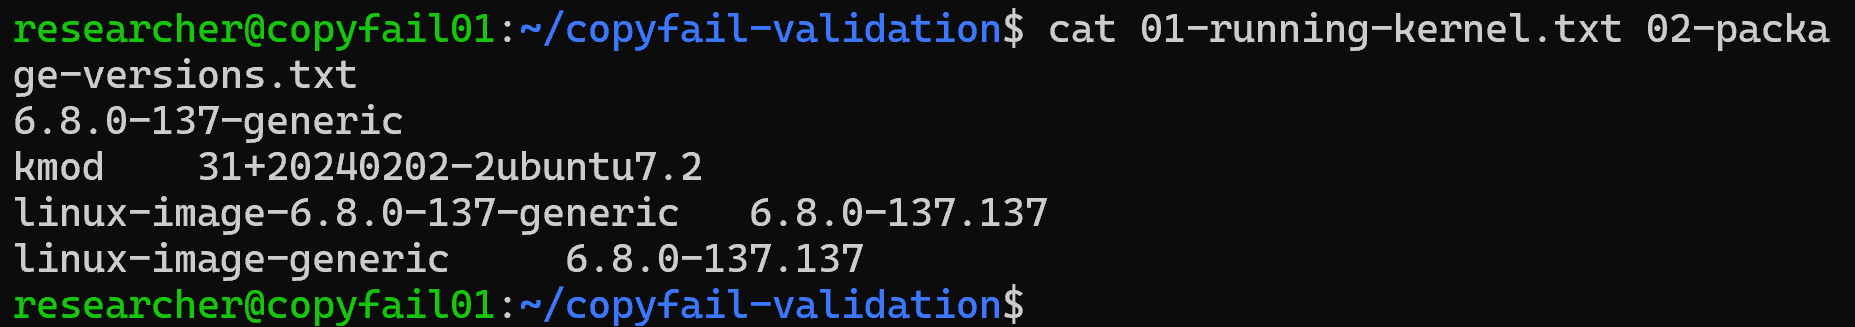
\includegraphics[
        width=\textwidth,
        height=0.29\textheight,
        keepaspectratio
    ]{01-vulnerability-validation/screenshots/02-patched-kernel-and-kmod.png}
    \caption{Running release and installed package versions recorded on
    VM~270 during Phase~01.}
    \label{fig:phase01-kernel-packages}
\end{figure}

Canonical identifies \code{6.8.0-117.117} as the first fixed version of the
Ubuntu 24.04 LTS Noble generic \code{linux} package
\cite{ubuntu-copyfail-cve}. The active \code{6.8.0-137.137} image is a later
update in that same maintained package series. VM~270 is therefore classified
as running a corrected vendor package.

This conclusion is based on the recorded runtime and package state together
with Canonical's published fixed-version boundary. It is not an independent
source-code review or binary comparison of the kernel image. That distinction
matters: the evidence supports a vendor-package classification, not a claim that
the patch was reimplemented or reverse engineered during this project.

\subsection{Combined Result}

The validation produces a layered result rather than a single yes-or-no module
check:

\begin{table}[H]
    \centering
    \caption{Copy Fail prerequisite assessment for VM~270.}
    \label{tab:reference-system-validation}
    \small
    \begin{tabularx}{\textwidth}{@{}>{\bfseries\raggedright\arraybackslash}p{0.29\textwidth}>{\raggedright\arraybackslash}p{0.17\textwidth}Y@{}}
        \toprule
        Property & Observation & What the evidence establishes \\
        \midrule
        Module object present &
        Yes &
        \code{algif\_aead.ko.zst} exists for the active release. \\

        AEAD userspace API configured &
        Yes, as a module &
        \code{CONFIG\_CRYPTO\_USER\_API\_AEAD=m} enables modular support. \\

        Module loaded at capture &
        No &
        The exact-name runtime query returned no row. \\

        Ordinary loading path permitted &
        No &
        \code{modprobe} resolves the requested insertion to
        \code{/bin/false}. \\

        Active kernel before fixed boundary &
        No &
        \code{6.8.0-137.137} is within the same Noble generic series and later
        than Canonical's fixed version, \code{6.8.0-117.117}. \\

        Suitable for direct reproduction &
        No &
        The captured reference state has both a module-loading control and a
        vendor-classified corrected kernel. \\
        \bottomrule
    \end{tabularx}
\end{table}

The module object and kernel support are present, but presence is not the same
as reachability or vulnerability. At collection time the module was unloaded,
the normal loading path was blocked, and the active kernel package was already
past the published correction boundary. VM~270 is therefore a protected
reference system, not a valid direct reproduction target.

No proof of concept was run on VM~270, so this chapter does not report an
observed exploit failure. Its conclusion is narrower and better supported: the
captured machine does not satisfy the prerequisites selected for the controlled
reproduction. Later protected-state retests remain separate experiments.

\subsection{Preserving the Reference System}

VM~270 was kept in its reference role instead of being downgraded or having its
module policy removed. Chapter~3 records the corresponding Proxmox state: the
machine was stopped and the current state descended from the
\code{clean-baseline-00} snapshot at the verification point. Preserving that
state keeps three later comparisons meaningful: vulnerable behaviour on
VM~271, behaviour under compensating controls, and behaviour after the vendor
kernel correction.

This also keeps experimental changes on the machine created for them. VM~271
\code{copyfail-vuln} is the clone on which the vulnerable kernel, necessary
module-policy change, proof of concept, detector, and compensating controls are
introduced. Its cloned machine identifiers and SSH host keys must be regenerated
before use, as specified in Chapter~2.

\subsection{Requirements for the Vulnerable Clone}

The reference-system result defines what must be shown on VM~271 before any
proof-of-concept execution:

\begin{table}[H]
    \centering
    \caption{Pre-reproduction acceptance criteria for VM~271.}
    \label{tab:vulnerable-clone-requirements}
    \small
    \begin{tabularx}{\textwidth}{@{}>{\bfseries\raggedright\arraybackslash}p{0.30\textwidth}Y@{}}
        \toprule
        Requirement & Evidence required before reproduction \\
        \midrule
        Candidate vulnerable kernel &
        Record the running release and exact installed image, module, and
        metapackage versions. \\

        Module mitigation absent or disabled &
        Capture the relevant \code{modprobe.d} content and the effective
        \code{modprobe -n -v algif\_aead} resolution. \\

        Affected interface reachable &
        Confirm that \code{algif\_aead} exists, can be loaded, and exposes the
        AF\_ALG AEAD path required by the reproduction. \\

        Unprivileged test identity &
        Record \code{labuser}, its UID and groups, and the absence of existing
        administrative privilege. \\

        Clean target state &
        Record the ownership, mode, size, and SHA-256 digest of the selected
        SUID target before execution. \\

        Isolation and identity separation &
        Keep the guest on the isolated laboratory network and regenerate the
        identifiers inherited during cloning. \\

        Recoverable checkpoint &
        Preserve a pre-PoC snapshot and its associated evidence before the
        exploit is introduced or executed. \\
        \bottomrule
    \end{tabularx}
\end{table}

Kernel package \code{6.8.0-116.116} was selected as the reconstruction
candidate because it immediately precedes Canonical's first fixed Noble generic
version, \code{6.8.0-117.117}. That ordering identifies a candidate package;
it does not by itself prove that the guest booted it, exposed the required
interface, or reproduced the vulnerability. Those points require direct runtime
and experimental evidence from VM~271.

Chapter~5 therefore begins by validating that reconstructed runtime and the
clean pre-exploitation state. Only after those checks can a privilege change be
attributed to the intended Copy Fail experiment rather than to an unknown
kernel, an already modified target, or an account with pre-existing privilege.